\documentclass[12pt]{article}
\usepackage{amsthm,amssymb,amsfonts,amsmath,amstext,systeme,graphicx,float,tabularx}
\marginparwidth 0pt
\oddsidemargin -1.2 truecm
\evensidemargin  0pt 
\marginparsep 0pt
\topmargin -2.2truecm
\linespread{1}
\textheight 25.8 truecm
\textwidth 18.5 truecm
\newenvironment{remark}{\noindent{\bf Remark }}{\vspace{0mm}}
\newenvironment{remarks}{\noindent{\bf Remarks }}{\vspace{0mm}}
\newenvironment{question}{\noindent{\bf Question }}{\vspace{0mm}}
\newenvironment{questions}{\noindent{\bf Questions }}{\vspace{0mm}}
\newenvironment{note}{\noindent{\bf Note }}{\vspace{0mm}}
\newenvironment{summary}{\noindent{\bf Summary }}{\vspace{0mm}}
\newenvironment{back}{\noindent{\bf Background}}{\vspace{0mm}}
\newenvironment{conclude}{\noindent{\bf Conclusion}}{\vspace{0mm}}
\newenvironment{concludes}{\noindent{\bf Conclusions}}{\vspace{0mm}}
\newenvironment{dill}{\noindent{\bf Description of Dill's model}}{\vspace{0mm}}
\newenvironment{maths}{\noindent{\bf Mathematics needed}}{\vspace{0mm}}
\newenvironment{inst}{\noindent{\bf Instructions}}{\vspace{0mm}}
\newenvironment{notes}{\noindent{\bf Notes }}{\vspace{0mm}}
\newenvironment{theorem}{\noindent{\bf Theorem }}{\vspace{0mm}}
\newenvironment{example}{\noindent{\bf Example }}{\vspace{0mm}}
\newenvironment{examples}{\noindent{\bf Examples }}{\vspace{0mm}}
\newenvironment{topics}{\noindent{\bf Topics}}{\vspace{0mm}}
\newenvironment{outcomes}{\noindent{\bf Expected Learning Outcomes}}{\vspace{0mm}}
\newenvironment{lemma}{\noindent{\bf Lemma }}{\vspace{0mm}}
\newenvironment{solution}{\noindent{\it Solution}}{\vspace{2mm}}
\newcommand{\ds}{\displaystyle}
\newcommand{\un}{\underline}
\newcommand{\bs}{\boldsymbol}

\begin{document}

\baselineskip 18 pt
\begin{center}
	{\large \bf ASGS By Topic}
\end{center}
\vspace{0.05cm}

\begin{enumerate}
	\item \textbf{HKDSE MATH Core Practice Paper I Q19}\\
	The amount of investment of a commercial firm in the 1st year is \$4 000 000. The amount of investment in each successive year is $r \%$ less than the previous year. The amount of investment in the 4th year is \$1 048 576.
	\begin{enumerate}
		\item[(a)] Find $r$. \\(2 marks)
		\item[(b)] The revenue made by the firm in the 1st year is \$2 000 000. The revenue made in each successive year is 20\% less than the previous year.
		\begin{enumerate}
			\item[(i)] Find the least number of years needed for the total revenue made by the firm to exceed \$9 000 000.
			\item[(ii)] Will the total revenue made by the firm exceed \$10 000 000? Explain your answer.
			\item[(iii)] The manager of the firm claims that the total revenue made by the firm will exceed the total amount of investment. Do you agree? Explain your answer.	
		\end{enumerate}
		(10 marks)
	\end{enumerate}

	\item \textbf{HKDSE MATH Core Sample Paper I Q15}\\
	The seats in a theatre are numbered in numerical order from the first row to the last row, and from left to right, as shown in Figure 7. The first row has 12 seats. Each succeeding row has 3 more seats than the previous one. If the theatre cannot accommodate more than 930 seats, what is the greatest number of rows of seats in the theatre? \\(4 marks)
	\begin{figure}[H]
		\centering
		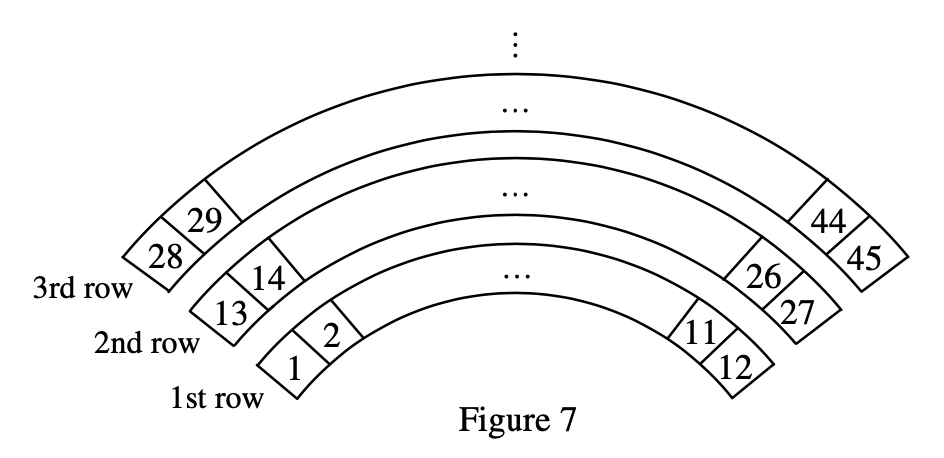
\includegraphics[width = .5\linewidth]{SPFigure1.7}
	\end{figure}





	\item \textbf{HKDSE MATH CORE 2012 Past Paper I Q19}\\
	In a city, the air cargo terminal $X$ of an airport handles goods of weight $A(n)$ tonnes in the $n$th year since the start of its operation, where $n$ is a positive integer. It is given that $A(n) = ab^{2n}$, where $a$ and $b$ are positive constants. It is found that the weights of the goods handled by $X$ in the 1st year and the 2nd year since the start of its operation are 254 100 tonnes and 307 461 tonnes respectively.
	\begin{enumerate}
		\item[(a)]
		\begin{enumerate}
			\item[(i)] Find $a$ and $b$. Hence find the weight of the goods handled by $X$ in the 4th year since the start of its operation.
			\item[(ii)] Express, in terms of $n$, the total weight of the goods handled by $X$ in the first $n$ years since the start of its operation.
		\end{enumerate}
		(6 marks)
		\item[(b)] The air cargo terminal $Y$ starts to operate since $X$ has been operated for 4 years. Let $B(m)$ tonnes be the weight of the goods handled by $Y$ in the $m$th year since the start of its operation, where $m$ is a positive integer. It is given that $B(m) = 2ab^m$.
		\begin{enumerate}
			\item[(i)] The manager of the airport claims that after $Y$ has been operated, the weight of the goods handled by $Y$ is less than that handled by $X$ in each year. Do you agree? Explain your answer.
			\item[(ii)] The supervisor of the airport thinks that when the total weight of the goods hangled by $X$ and $Y$ since the start of the operation of $X$ exceeds 20 000 000 tonnes, new facilities should be installed to maintain the efficiency of the air cargo terminals. According to the supervisor, in which year since the start of the operation of $X$ should the new facilities be installed?
		\end{enumerate}
		(7 marks)
	\end{enumerate}

	\item \textbf{HKDSE MATH CORE 2013 Past Paper I Q19}\\
	The development of public housing in a city is under study. It is given that the total floor area of all public housing at the end of the 1st year is $9 \times 10^6$ m$^2$ and in subsequent years, the total floor area of public housing flats built each year is $r$ $\%$ of the total floor area of all public housing flats at the end of the previous year, where r is a constant, and the total floor area of public housing flats pulled down each year is $3 \times 10^5$ m$^2$. It is found that the total floor area of all public housing flats at the end of the 3rd year is $1.026 \times 10^7$ m$^2$.
	\begin{enumerate}
		\item[(a)]
		\begin{enumerate}
			\item[(i)] Express, in terms of $r$, the total floor area of all public housing flats at the end of the 2nd year.
			\item[(ii)] Find $r$.
		\end{enumerate}
		(4 marks)
		\item[(b)]
		\begin{enumerate}
			\item[(i)] Express, in terms of $n$, the total floor area of all public housing flats at the end of the $n$th year.
			\item[(ii)] At the end of which year will the total floor area of all public housing flats first exceed $4 \times 10^7$ m$^2$?
		\end{enumerate}
		(5 marks)
		\item[(c)] It is assumed that the total floor area of public housing flats needed at the end of the $n$th year is $(a(1.21)^n + b)$ m$^2$, where $a$ and $b$ are constants. Some research results reveal the following information:
		$$\begin{array}{|c|c|}
			\hline
			n & \text{The total floor area of public housing flats needed at the end of the $n$th year (m$^2$)} \\
			\hline
			1 & 1 \times 10^7\\
			\hline		
			2 & 1.063 \times 10^7\\
			\hline
		\end{array}$$		
		A research assistant claims that based on the above information, the total floor area of all public housing flats will be greater than the total floor area of public housing flats needed at the end of a certain year. Is the claim correct? Explain your answer. \\(4 marks)
	\end{enumerate}


    \item \textbf{HKDSE MATH CORE 2014 Past Paper I Q16}\\
	In figure 5, the 1st pattern consists of 3 dots. For any positive integer $n$, the $(n + 1)$th pattern is formed by adding 2 dots to the nth pattern. Find the least value of m such that the total number of dots in the first $m$ patterns exceeds 6 888. \\(4 marks)
	\begin{figure}[H]
		\centering
		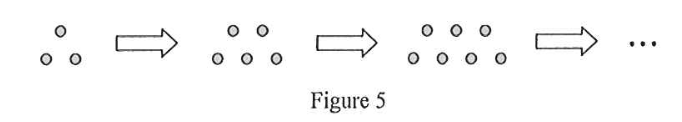
\includegraphics[width = .6\linewidth]{2014Figure1.5}
	\end{figure}

    \item \textbf{HKDSE MATH CORE 2015 Past Paper I Q17}\\
	For any positive integer $n$, let $A(n) = 4n - 5$ and $B(n) = 10^{4n-5}$.
	\begin{enumerate}
		\item[(a)] Express $A(1) + A(2) + A(3) + \cdots + A(n)$ in terms of $n$. \\(2 marks)
		\item[(b)] Find the greatest value of n such that $\log{(B(1)B(2)B(3)\cdots B(n))}\leq 8000$. \\(3 marks)
	\end{enumerate}

    \item \textbf{HKDSE MATH CORE 2016 Past Paper I Q17}\\
	The 1st term and the 38th term of an arithmetic sequence are 666 and 555 respectively. Find
	\begin{enumerate}
		\item[(a)] the common difference of the sequence, \\(2 marks)
		\item[(b)] the greatest value of n such that the sum of the first n terms of the sequence is positive. \\(3 marks)
	\end{enumerate}


	\item \textbf{HKDSE MATH CORE 2017 Past Paper I Q16}\\
	A city adopts a plan to import water from another city. It is given that the volume of water imported in the 1st year since the start of the plan is $1.5 \times 107$ m$^3$ and in subsequent years, the volume of water imported each year is 10\% less than the volume of water imported in the previous year.
	\begin{enumerate}
		\item[(a)] Find the total volume of water imported in the first 20 years since the start of the plan. \\(2 marks) 
		\item[(b)] Someone claims that the total volume of water imported since the start of the plan will not exceed $1.6 \times 108$ m$^3$. Do you agree? Explain your answer. \\(2 marks)
	\end{enumerate}

    \item \textbf{HKDSE MATH CORE 2018 Past Paper I Q16}\\
	The 3rd term and the 4th term of a geometric sequence are 720 and 864 respectively.
	\begin{enumerate}
		\item[(a)] Find the 1st term of the sequence. \\(2 marks)
		\item[(b)] Find the greatest value of $n$ such that the sum of the $(n + 1)$th term and the $(2n + 1)$th term is less than $5 \time 10^{14}$. \\(3 marks)
	\end{enumerate}

    \item \textbf{HKDSE MATH CORE 2019 Past Paper I Q16}\\
	Let $\alpha$ and $\beta$ be real numbers such that $\left\{\begin{matrix}
		\beta  =  5\alpha  -  18 \\
		\beta = \alpha^2 - 13\alpha + 63\\
		\end{matrix}\right.$ .
	\begin{enumerate}
		\item[(a)] Find $\alpha$ and $\beta$. \\(2 marks)
		\item[(b)] The 1st term and the 2nd term of an arithmetic sequence are $\log{\alpha}$ and $\log{\beta}$ respectively. Find the least value of $n$ such that the sum of the first $n$ terms of the sequence is greater than 888. \\(4 mark)
	\end{enumerate}

    \item \textbf{HKDSE MATH CORE 2020 Past Paper I Q16}\\
	The 3rd term and the 6th term of a geometric sequence are 144 and 486 respectively.
	\begin{enumerate}
		\item[(a)] Find the 1st term of the sequence. \\(2 marks) 
		\item[(b)] Find the least value of $n$ such that the sume of the first $n$ terms of the sequence is greater than $8 \times 10^{18}$. \\(3 marks)
	\end{enumerate}

    \item \textbf{HKDSE MATH CORE 2021 Past Paper I Q17}\\
	Let $A(n)$ be the $n$th term of an arithmetic sequence. It is given that $A(5) = 26$ and $A(12) = 61$.
	\begin{enumerate}
		\item[(a)] Find $A(1)$. \\(2 marks)
		\item[(b)] Suppose that $\log_2{G(n)} = A(n)$ for any positive integer $n$. Find the greatest value of $k$ such that $\log_8{\left(G(1)G(2)G(3)\cdots G(k)\right) < 999}$. \\(5 marks)
	\end{enumerate}

    \item \textbf{HKDSE MATH CORE 2022 Past Paper I Q17}\\
	Let $c$ be a real constant. The roots of the equation $x^2 + cx - 9 = 0$ are $\alpha$ and $\beta$.
	\begin{enumerate}
		\item[(a)] Express $\alpha^2 + \beta^2$ in terms of $c$. \\(3 marks)
		\item[(b)] The 1st term, the 2nd term and the 3rd term of an arithmetic sequence are $c^2$, $\alpha^2 + \beta^2$ and 85 respectively. Find the least value of $n$ such that the sum of the first $n$ terms of the sequence is greater than $2 \times 10^6$. \\(4 marks)
	\end{enumerate}

    \item \textbf{HKDSE MATH CORE 2023 Past Paper I Q18}\\
	Suppose that $\alpha , 7 , \beta $ is a geometric sequence, where $q < \alpha < \beta$.
	\begin{enumerate}
		\item[(a)] Express $\log_7{\alpha}$ in terms of $\log_7{\beta}$. \\(3 marks)
		\item[(b)] If $\log_{\beta}{\alpha}, \log_{7}{\beta}, \log_{\alpha}{\beta}$ is an arithmetic sequence, find the common difference of the arithmetic sequence. \\(5 marks)
	\end{enumerate}


\end{enumerate}








\end{document}